%%%%%%%%%%%%%%%%%%%%%%%%%%%%%%%%%%%%%%%%%%%%%%
%Lab report writeup based on template by Derek Hildreth
%%%%%%%%%%%%%%%%%%%%%%%%%%%%%%%%%%%%%%%%%%%%%%

%\documentclass[aps,letterpape,10pt]{revtex4}
\documentclass[aps,letterpaper,10pt]{article}
%\documentclass{article}

\usepackage{graphicx} % For images
\usepackage{float}    % For tables and other floats
\usepackage{verbatim} % For comments and other
\usepackage{amsmath}  % For math
\usepackage{amssymb}  % For more math
\usepackage{fullpage} % Set margins and place page numbers at bottom center
\usepackage{subfig}   % For subfigures
\usepackage[usenames,dvipsnames]{color} % For colors and names
\usepackage{fancyhdr} %headers
\usepackage{listings} %for code
\usepackage{color} %to color code
\usepackage{wrapfig} % for inline images

%Color and code setup
\definecolor{dkgreen}{rgb}{0,0.6,0}
\definecolor{gray}{rgb}{0.5,0.5,0.5}
\definecolor{mauve}{rgb}{0.58,0,0.82}
\definecolor{codebg}{rgb}{.95,.95,.98}

\lstset{ %
	language=Python, 
	tabsize=4, 
	numbers=left,
	numberstyle=\footnotesize,
	backgroundcolor=\color{codebg},
	breaklines=true,
	breakatwhitespace=true,
	basicstyle=\small,
	numberstyle=\tiny\color{black},
	showstringspaces=false,
	keywordstyle=\color{blue}, 
	stringstyle=\color{dkgreen},
	commentstyle=\color{gray},
	frame=single,
	title = \texttt{\lstname}
	}

%%%%%%%%%%%%

%HEADER FORMATING%%%%%%%%%%%%%
\pagestyle{fancy}
\headheight 10pt
\setlength{\headsep}{20pt}
\lhead{MPHY 396 - Prof. Suzuki\\ Homework 11}
\rhead{A. Athanassiadis\\Due 3/7/2012}
%%%%%%%%%%%%%%%%%%%%%%%%

%Custom Definitions%%%%%%%%%%%%%%%
\newcommand{\ttt}{\texttt}
%%%%%%%%%%%%%%%%%%%%%%%%

\begin{document}


\section{Problem 1}
\textbf{Prove that the set of first principal components has maximum variance among any other set of principal components.}\\

Consider a data set $X=\{x^{(\mu)} \mid \mu\in[1,P]\}$ in an $N$ dimensional feature space. Let $C=XX^T$ be the covariance of $X$, and $\phi^{(i)}$ the eigenvectors of the linear equation $C\phi^{(i)} = \lambda_i\phi^{(i)}$ with eigenvectors $\lambda_i$ for $i\in[1,N]$. Furthermore, order $(\lambda_i, \phi^{(i)})$ such that for $i>k$ we have $\lambda_i<\lambda_k$. Furthermore let $a_i^{(\mu)}$ be the $i$-th principal component of $x^{(\mu)}$ given by $a_i^{(\mu)} = \langle{x^{(\mu)}, \phi^{(i)}}\rangle$.

$a_i^{(\mu)}$ is thus a projection of $x^{(\mu)}$ onto the eigenvector $\phi^{(i)}$. The variance of $a_i$ is thus the variance of $X$ with respect to the $i$-th eigenvector.  Since the eigenvectors $\{\phi^{(i)}\}$ are of the covariance of $X$, the covariance of $X$ with respect to any $\phi^{(i)}$ is a diagonal matrix and is equal to the variance of $X$ with respect to the same eigenvector. Therefore, $\text{Var}(a_i) = \text{Cov}(X)_{\phi^{(i)}} = \lambda_i$.  By hypothesis, $\lambda_1>\lambda_i\, \forall i>1$.  Therefore $\text{Var}(a)$ is maximal along the first principal component.

Heuristically, the first principal component is constructed to be the component along which the covariance of $X$ is maximal. Therefore, the projection of the data set $X$ onto the different components, which is denoted by $a_i$, has maximal variance along the first principal component, since the variance of $X$ along the component is equal to the covariance with respect to that component.

\newpage
\section{Problem 2}
\textbf{Calculate and display eigenfaces as well as approximation faces.}\\

Using the script below and \ttt{eigenface.py}, I performed PCA on the set of faces supplied. Figure \ref{fig:11-2a} shows the average face, and Figure \ref{fig:11-2b} show the first eight eigenfaces (in order) determined from the data set. Figure \ref{fig:11-2c} shows the first face given in the set, and Figure \ref{fig:11-2d} shows the first eight approximation eigenfaces.

\lstinputlisting{problem2.py}

\begin{figure}[!p]
\centering
\begin{minipage}{.3\textwidth}
\centering
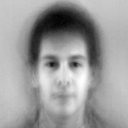
\includegraphics[width=\textwidth]{eigenfaces/avgface.png}
\caption{Average Face}
\label{fig:11-2a}
\end{minipage}
\begin{minipage}{.75\textwidth}
\centering
\subfloat[]{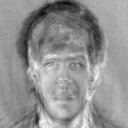
\includegraphics[width=.3\textwidth]{eigenfaces/eigenface0.png}}\hfill
\subfloat[]{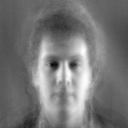
\includegraphics[width=.3\textwidth]{eigenfaces/eigenface1.png}}\hfill
\subfloat[]{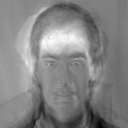
\includegraphics[width=.3\textwidth]{eigenfaces/eigenface2.png}}\\
\subfloat[]{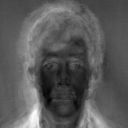
\includegraphics[width=.3\textwidth]{eigenfaces/eigenface3.png}}\hfill
\subfloat[]{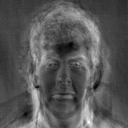
\includegraphics[width=.3\textwidth]{eigenfaces/eigenface4.png}}\hfill
\subfloat[]{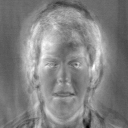
\includegraphics[width=.3\textwidth]{eigenfaces/eigenface5.png}}\\
\subfloat[]{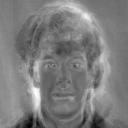
\includegraphics[width=.3\textwidth]{eigenfaces/eigenface6.png}}\hfill
\subfloat[]{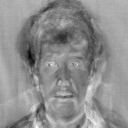
\includegraphics[width=.3\textwidth]{eigenfaces/eigenface7.png}}
\caption{First 8 eigenfaces}
\label{fig:11-2b}
\end{minipage}
\end{figure}

\begin{figure}[!p]
\centering
\begin{minipage}{.3\textwidth}
\centering
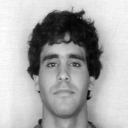
\includegraphics[width=\textwidth]{face_approx/original.png}
\caption{Input Face}
\label{fig:11-2c}
\end{minipage}
\begin{minipage}{.75\textwidth}
\centering
\subfloat[]{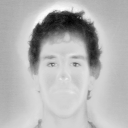
\includegraphics[width=.3\textwidth]{face_approx/approx1.png}}\hfill
\subfloat[]{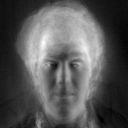
\includegraphics[width=.3\textwidth]{face_approx/approx2.png}}\hfill
\subfloat[]{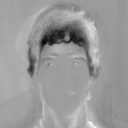
\includegraphics[width=.3\textwidth]{face_approx/approx3.png}}\\
\subfloat[]{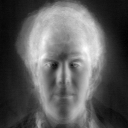
\includegraphics[width=.3\textwidth]{face_approx/approx4.png}}\hfill
\subfloat[]{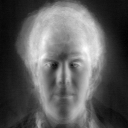
\includegraphics[width=.3\textwidth]{face_approx/approx5.png}}\hfill
\subfloat[]{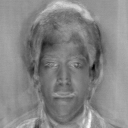
\includegraphics[width=.3\textwidth]{face_approx/approx6.png}}\\
\subfloat[]{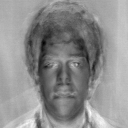
\includegraphics[width=.3\textwidth]{face_approx/approx7.png}}\hfill
\subfloat[]{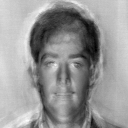
\includegraphics[width=.3\textwidth]{face_approx/approx8.png}}
\caption{First 8 approximation faces}
\label{fig:11-2d}
\end{minipage}
\end{figure}


\newpage
\section{Appendix: Common Code}
The base code used for Problem 1 in this homework is contained in \ttt{eigenface.py}.
\lstinputlisting{eigenface.py}
\end{document} 
